\documentclass[tikz,border=2pt]{standalone}
\usepackage{amsmath,amssymb}
\usetikzlibrary{arrows.meta}

\begin{document}
% The bounded interval [a, b] on the real line, with its left endpoint a and right endpoint b.
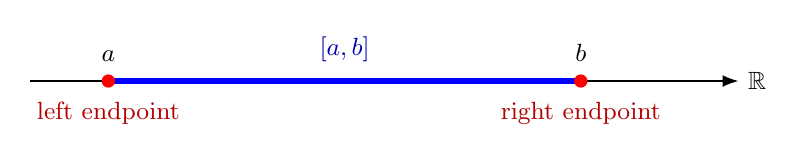
\begin{tikzpicture}[every node/.style={font=\small}, >={Latex[length=2mm]}]
	\draw[->] (-1,0) -- (8,0) node[right] {$\mathbb R$};
	\draw[blue, line width=2pt] (0,0) -- (6,0);
	\fill[red] (0,0) circle (2.4pt);
	\fill[red] (6,0) circle (2.4pt);
	\node[anchor=south] at (0,0.12) {$a$};
	\node[anchor=south] at (6,0.12) {$b$};
	\node[anchor=north, red!70!black, font=\small] at (0,-0.15) {left endpoint};
	\node[anchor=north, red!70!black, font=\small] at (6,-0.15) {right endpoint};
	\node[blue!70!black, anchor=south] at (3,0.12) {$[a,b]$};
\end{tikzpicture}
\end{document}
